\section*{Question 2}
\fakesection{2}

This problem upsamples the downsampled signal of Question 1 back to the original sampling rate. We compare separately upsampling then filtering versus applying a polyphase interpolator.

First, we separately upsample then filter. The signal shown in Figure \ref{fig:q1_polydecimate} is zero-packed with $L-1=79$ zeros between each element to get back the original sampling rate of 40 kHz.

\begin{figure}[ht]
    \centering
    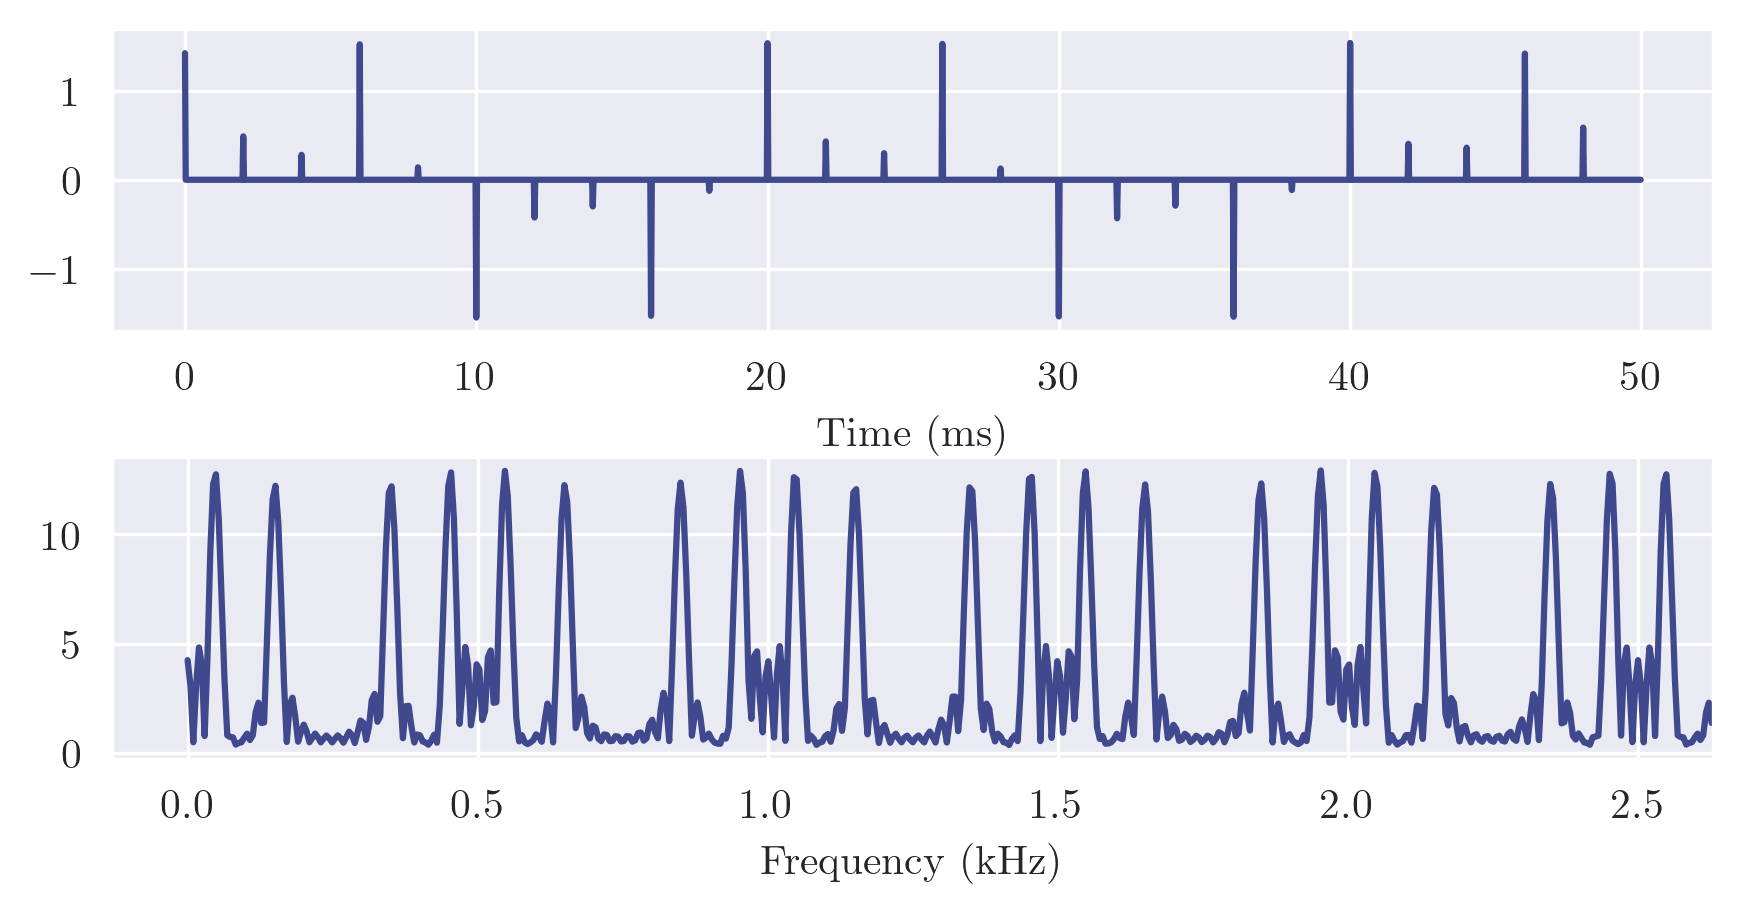
\includegraphics[width=\textwidth]{images/q2_zpack.png}
    \caption{Zero-packed signal upsampled by $L$=80 back to 40 kHz}
    \label{fig:q2_zpack}
\end{figure}

Zero-packing produces undesirable copies of the frequency spectrum, which we remove using the Kaiser-windowed low pass filter from Question 1.

\begin{figure}[ht]
    \centering
    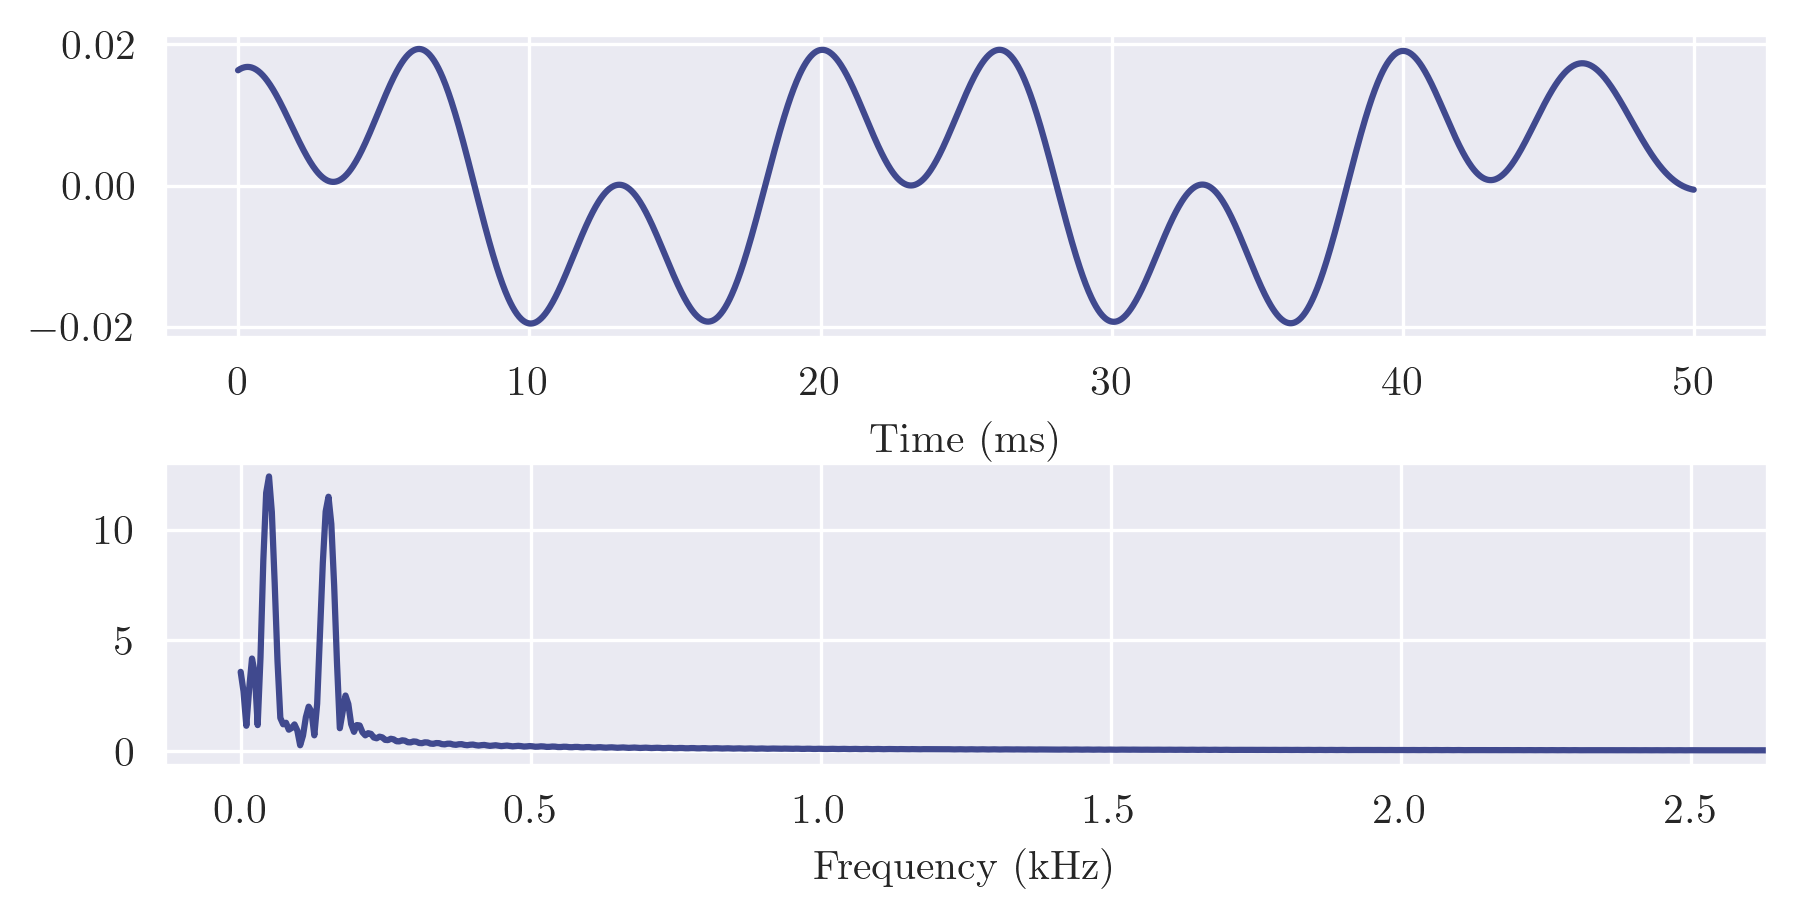
\includegraphics[width=\textwidth]{images/q2_usamp.png}
    \caption{Zero-packed signal filtered to contain only 50 and 150 Hz tones}
    \label{fig:q2_usamp}
\end{figure}

Comparing Figure \ref{fig:q2_usamp} to Figure \ref{fig:q1_filtered} from Question 1, we observe that we have successfully upsampled then filtered the signal.

Now we try a polyphase interpolator. This involves:
\begin{enumerate}
    \item Zero-padding the LPF coefficients to a multiple of $L$.
    \item Reshaping the the LPF coefficients into a column-major matrix with $L$ rows.
    \item Convolving each row of filter coefficients with the entire input signal.
    \item Constructing a row-major matrix from the resulting $L$ convolution outputs.
    \item Flattening the matrix column-wise into a vector representing the output signal.
\end{enumerate}
After removing transient edge effects, the overall output signal is a factor of $L$ longer than the input signal. The output is shown in Figure \ref{fig:q2_polyinterpolate}.

\begin{figure}[ht]
    \centering
    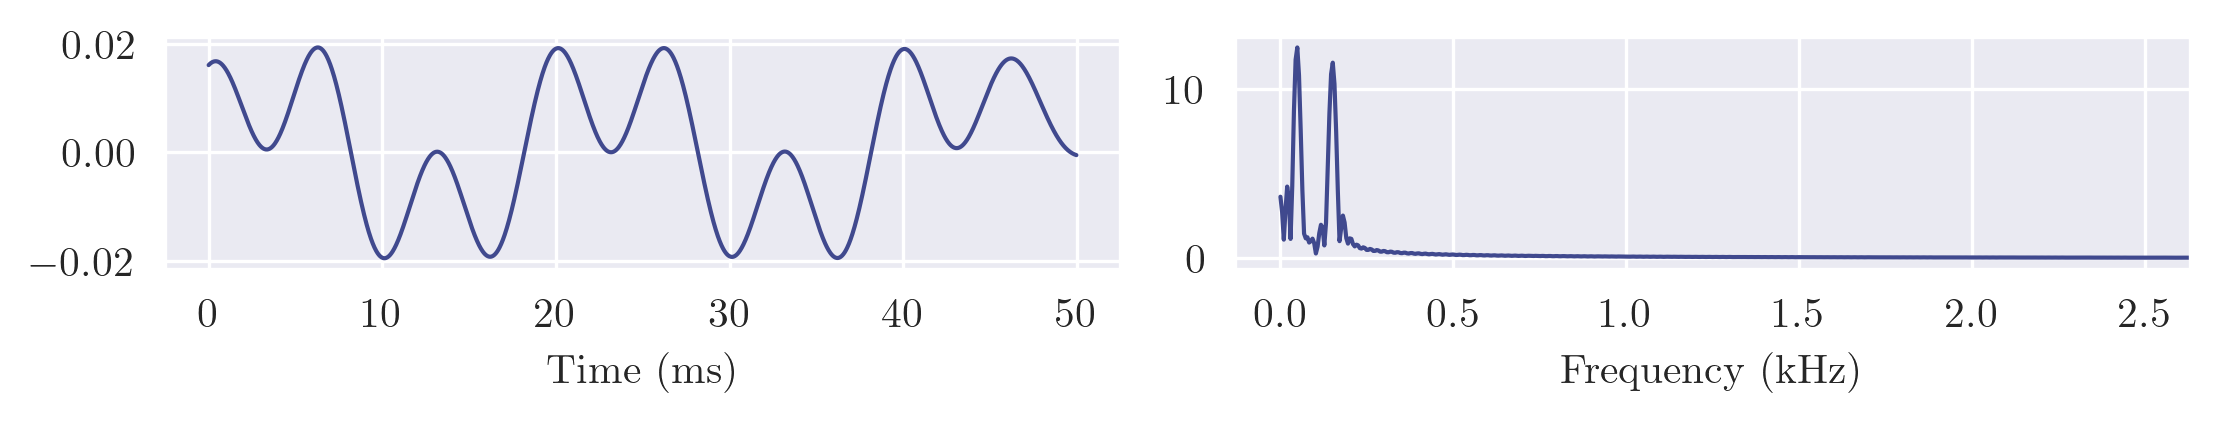
\includegraphics[width=\textwidth]{images/q2_polyinterpolate.png}
    \caption{Polyphase interpolator applied to downsampled signal of Question 1}
    \label{fig:q2_polyinterpolate}
\end{figure}

\newpage

The output is the same as separately upsampling then filtering, and also equal to the original signal of Figure \ref{fig:q1_filtered}. Yet the second noble identity states that the polyphase filter requires $L$ times less computations. Intuitively, by upsampling before filtering, $L-1$ upsampled elements are zero, representing meaningless computations during filtering. Hence, by filtering before upsampling, the polyphase interpolator achieves a theoretical $L$-fold performance gain.

Similar to Question 1, we can test this by timing 10,000 trials of both methods. On average:
\begin{itemize}
    \item Upsample then filter: 1.529 ms
    \item Polyphase interpolator: 0.801 ms
\end{itemize}
In the same vein as Question 1, the polyphase filter is faster, though not by a factor of $L$. Optimising away the overhead of the polyphase filter is outside the scope of this problem.
